\begin{figure} [h]
         \centering
         \caption{ lorem ipsum }
         \label{fig:1}
         \centering
         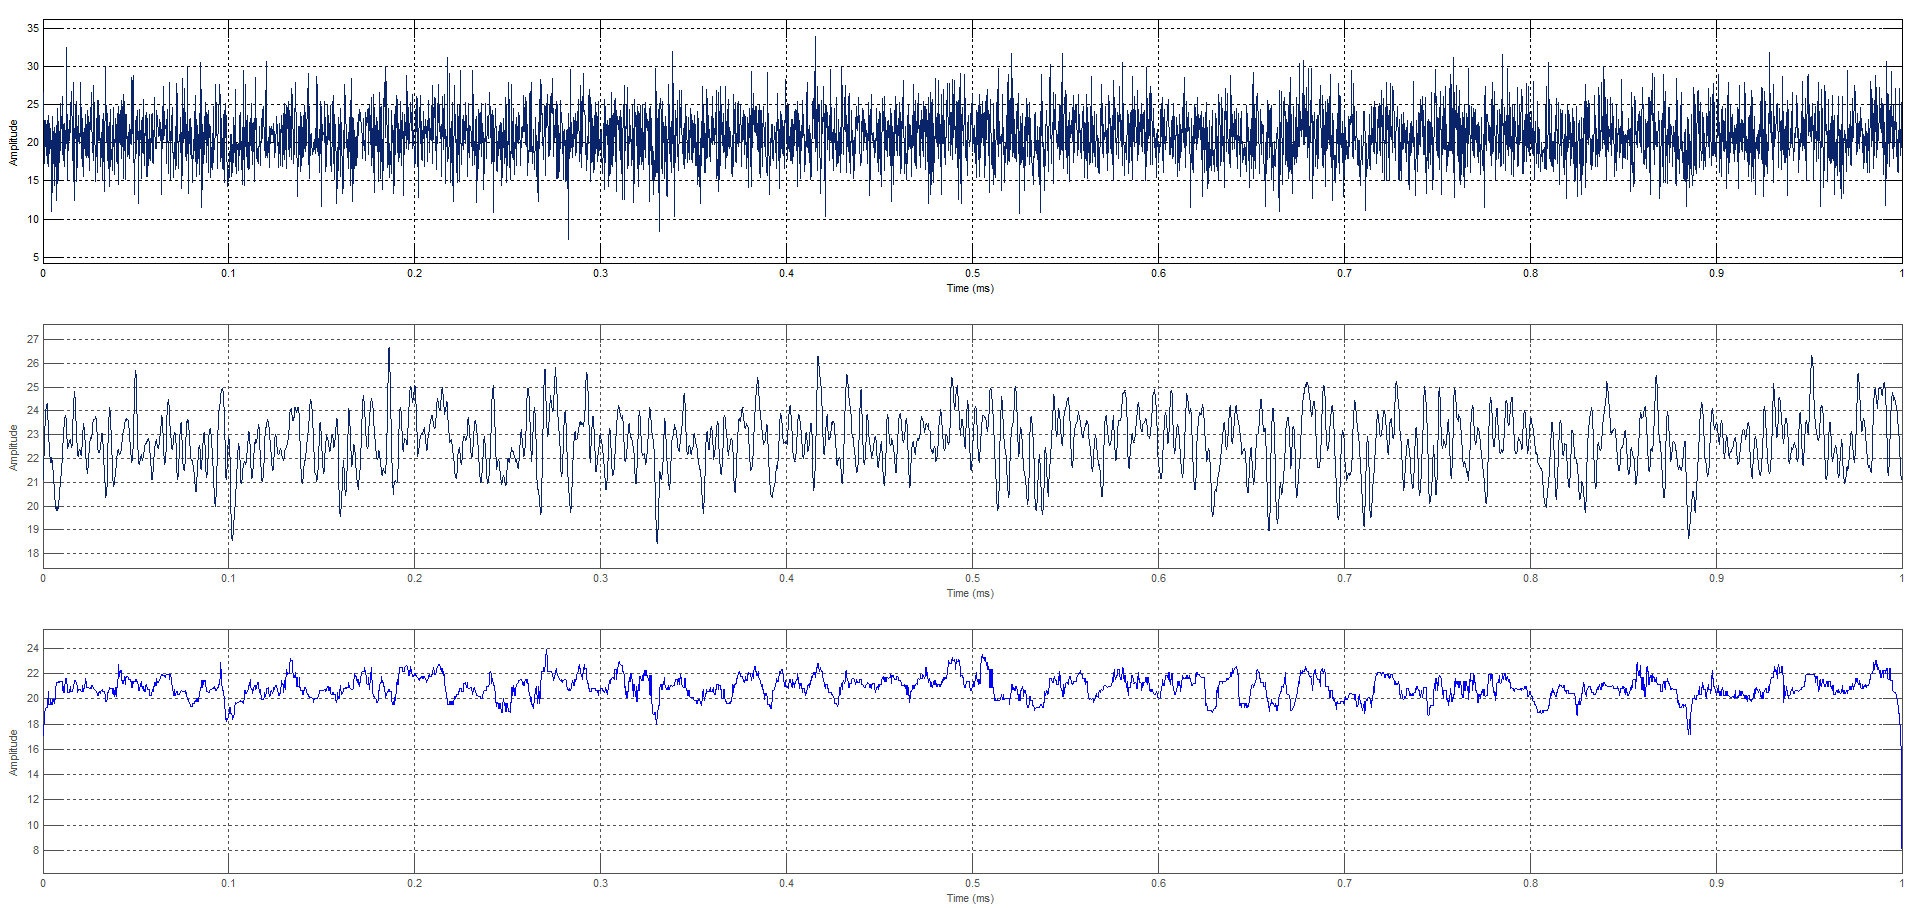
\includegraphics[width=.8\textwidth]{common/img/AmpGefiltert_small.png}

\end{figure}
%---------------------------------------------------------------------------------------
\vspace{.5cm}
%---------------------------------------------------------------------------------------
\begin{figure} [h]
         \centering
         \caption{ Spektrum des Messsignals, vor und nach der Filterung  }
         \label{fig:2}
	     \centering
	     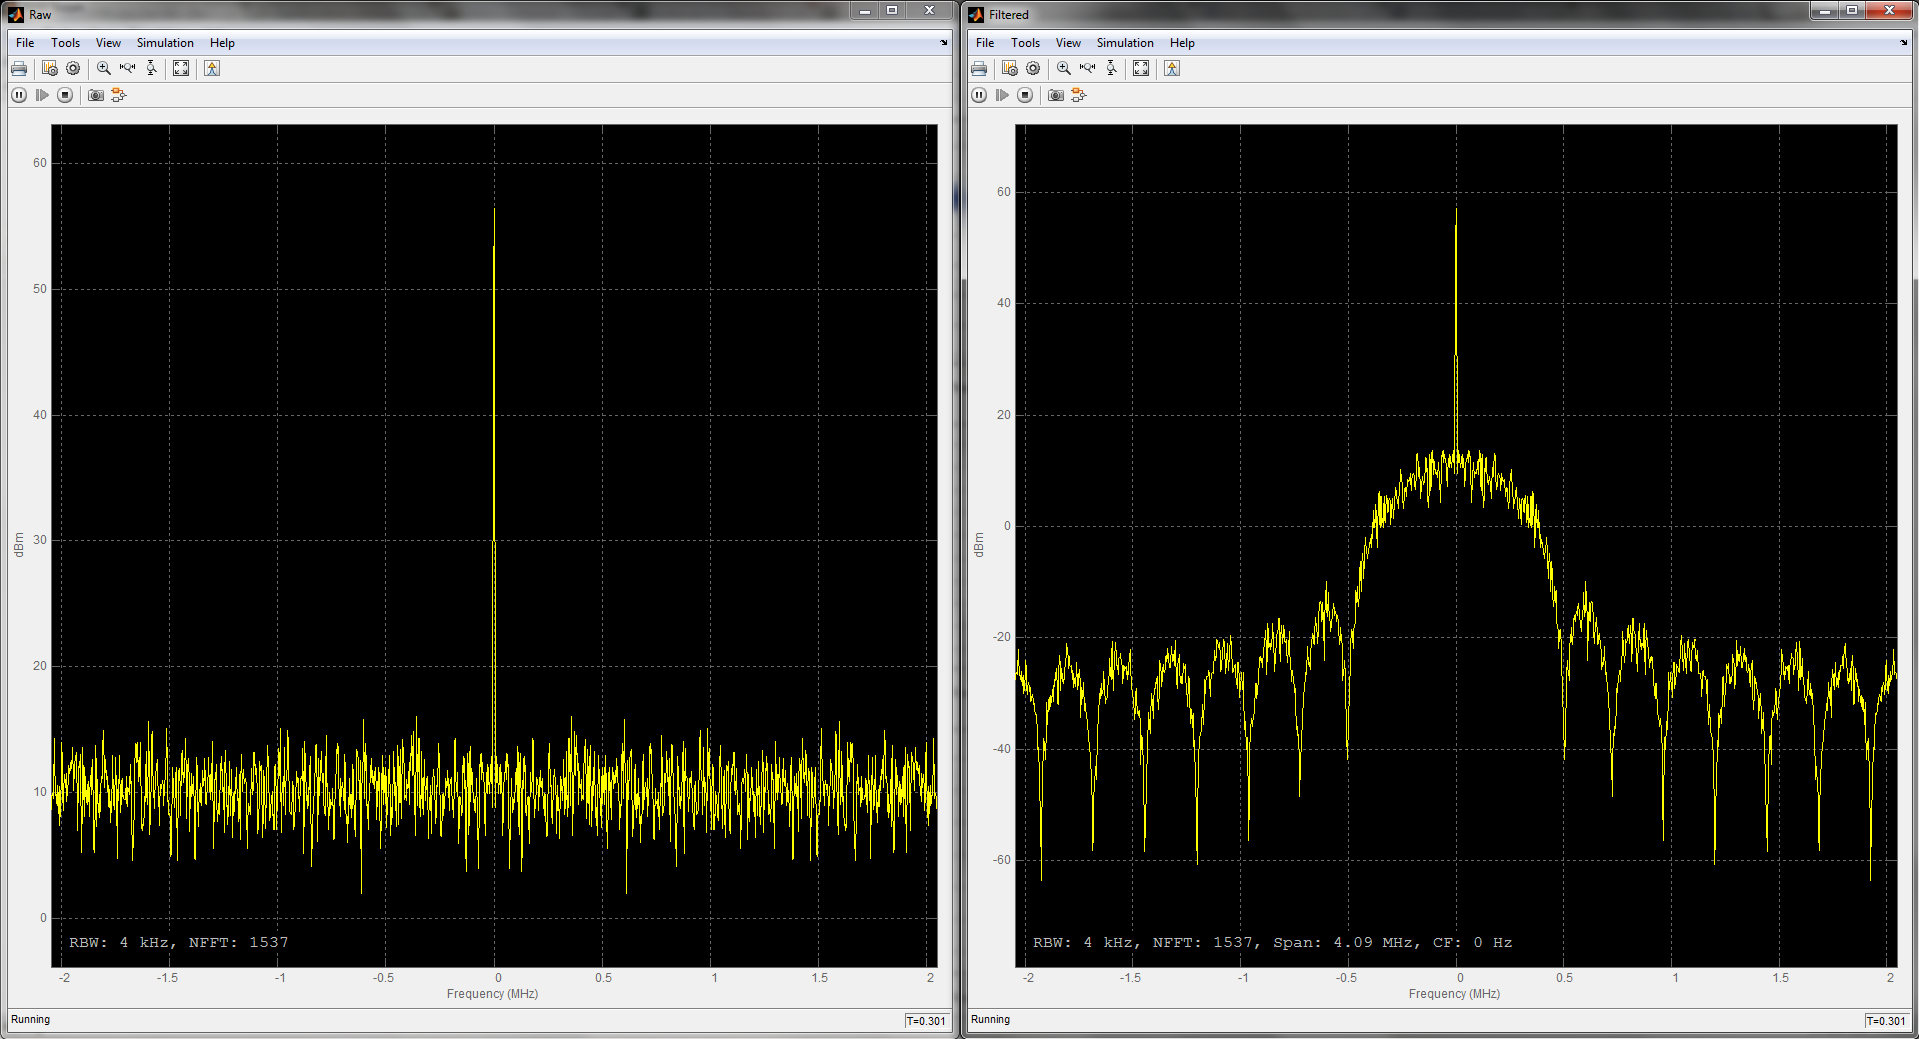
\includegraphics[width=.6\textwidth]{common/img/SpektrumAmp.PNG} \\
\vspace{.2cm}
Die Grafik zeigt das Spektrum des Messsignals der Amplitude. Im linken Bild ist das ungefilterte Signal und im Rechten das gefilterte.
%
\end{figure}
%---------------------------------------------------------------------------------------
\vspace{.5cm}
%---------------------------------------------------------------------------------------
\begin{figure} [h]
         \centering
         \caption{ Frequenzgänge der entworfenen Filter. Beide ähneln sich in den Parametern, verfügen jedoch über etwas unterschiedliche Eckfrequenzen. Als Entwurfsmethode wurde die sog. "Least-squares"-Methode verwendet. Diese Methode liefert gute Ergebnisse im Hinblick auf aöglichst kleine Sidelobes und eine geringe Anzahl an Taps. }
         \label{fig:3}
%         
         \begin{subfigure}[t]{0.5\textwidth}
                 \centering
                 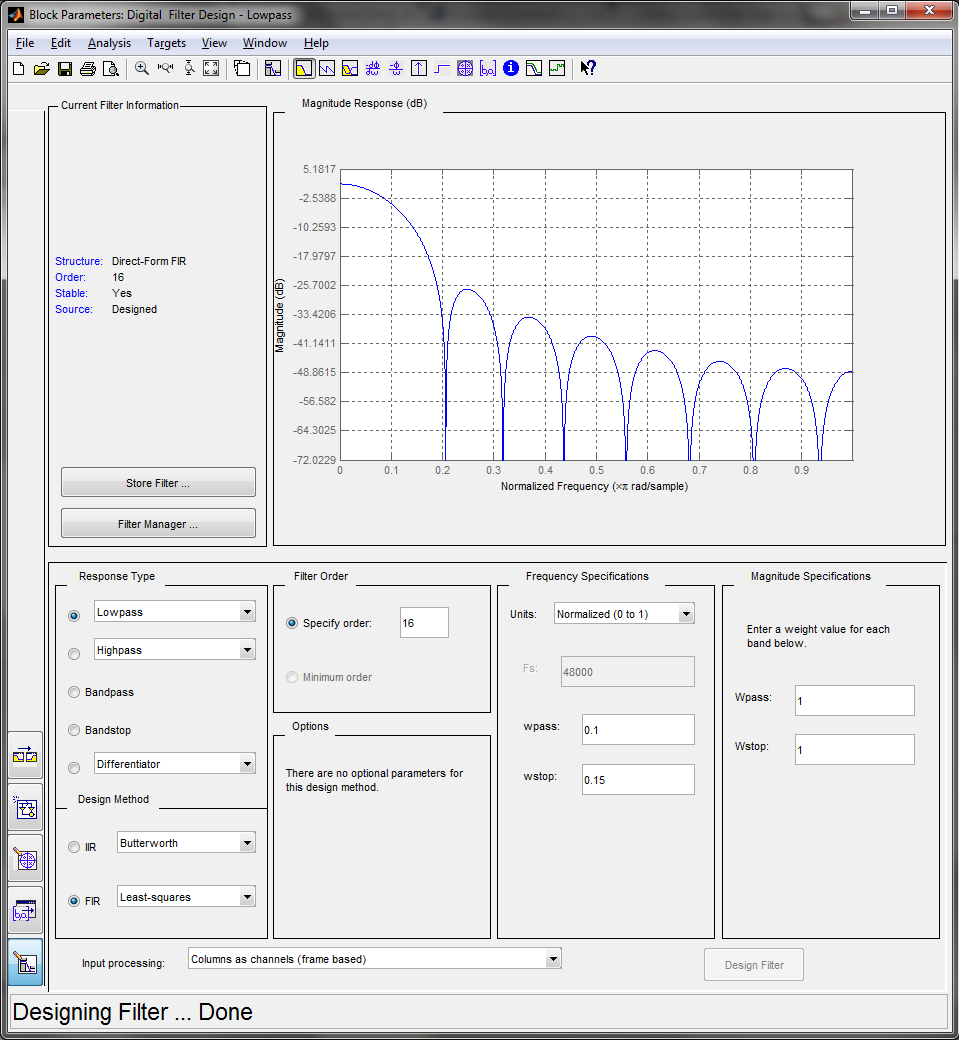
\includegraphics[width=\textwidth]{common/img/filter.png}
                 \vspace{.1cm}
                 \caption{Erstes Filter mit den Parametern wpass~=~0.1 und wstop~=~0.15. Das Ergebnis ist ein schmalbandigeres Filter. }
                 \label{fig:Filter1_A}\textit{}
         \end{subfigure}
%         
\qquad
         \begin{subfigure}[t]{0.5\textwidth}
                 \centering
                 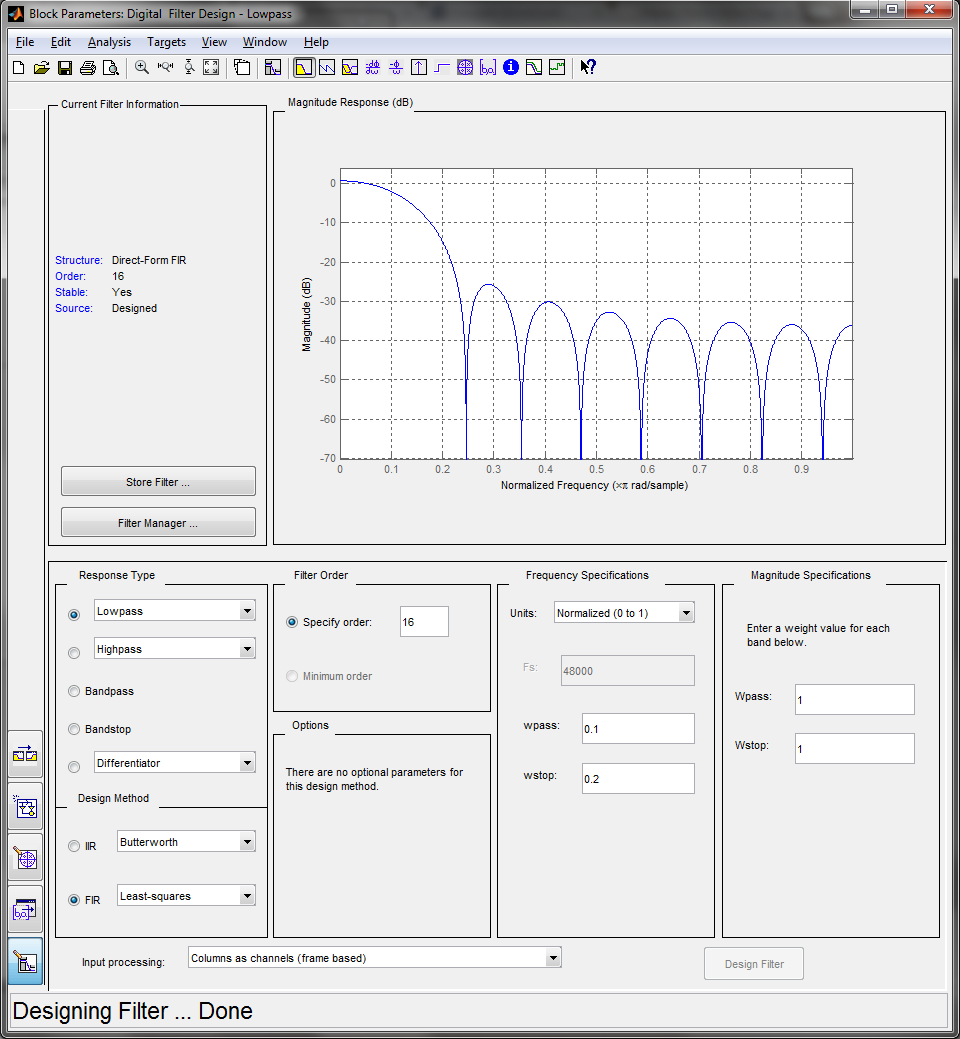
\includegraphics[width=\textwidth]{common/img/filter2.png}
                 \vspace{.1cm}
                 \caption{ Zweites Filter mit den Parametern wpass~=~0.1 und wstop~=~0.2. Der Durchlas bereich ist etwas breit, dafür sind die Sidelobes besser gedämpft }
                 \label{fig:Filter2_B}
         \end{subfigure}
%
\end{figure}
%---------------------------------------------------------------------------------------